\documentclass[conference,onecolumn]{IEEEtran}
\IEEEoverridecommandlockouts
\ifCLASSINFOpdf
\else
  \usepackage[dvips]{graphicx}
  \graphicspath{{./}}
  \DeclareGraphicsExtensions{.eps}
\fi

\usepackage[cmex10]{amsmath}
\usepackage{algorithm}
\usepackage{algorithmic}
\usepackage{array}
\usepackage{url}

% correct bad hyphenation here
\hyphenation{op-tical net-works semi-conduc-tor}

\begin{document}
\title{ROSS.Net: Large-scale Network Simulation for Mobile Ad-hoc Networks}

% author names and affiliations
% use a multiple column layout for up to three different
% affiliations
 \author{\IEEEauthorblockN{David W. Bauer Jr.}
 \IEEEauthorblockA{High Performance Technologies, Inc.\\
 Reston, VA 20190\\
 Email: dbauer@hpti.com}
 \and
 \IEEEauthorblockN{Christopher D. Carothers}
 \IEEEauthorblockA{Rensselaer Polytechnic Institute \\
 Troy, NY 12180 \\
 Email: chrisc@cs.rpi.edu}}

\maketitle

\section{Introduction}

\begin{figure}[!h]
\centering
\includegraphics[width=5in]{rn_combines.ps}
\caption{High level abstraction of the ROSS.Net architecture.  ROSS.Net aims to bring together the four major areas of network research: simulation, protocol design, measurement and experiment design.}
\label{fig-rn-arch}
\end{figure}

The ROSS.Net network simulation framework supports the study of large-scale network models on High Performance Computing (HPC) platforms.  This User's Guide serves to document the features, execution and extensibility of ROSS.Net.

As shown in Figure \ref{fig-rn-arch}, ROSS.Net aims to bring together four major areas of networking research: simulation, protocol design, network modeling and measurement and experiment design.  The major components of ROSS.Net are an experiment design framework, a parallel discrete event simulator, and efficient models for network protocols and layering \cite{yaun-2003-1,bauer-2003, bauer-2004}.

ROSS.Net incorporates the Unified Search Framework (USF) for performing optimization over the range of ROSS.Net parameters for the study of large-scale networks \cite{ye-2003}.  USF automates the process of experiment design and analysis.  For simulation, at the heart of ROSS.Net is Rensselaer's Optimistic Simulation System (ROSS). ROSS is a parallel discrete event, parallel execution simulation engine that has been shown to scale to tens of thousands of processors for synthetic benchmarks, as well as realistic models of mobility and waveforms for mobile ad-hoc networks \cite{bauer-2002}. Running on top of ROSS is the ROSS.Net simulation model. The ROSS.Net simulation model provides efficient mechanisms for layering multiple network protocol models, multiplexing packet streams, packet encapsulation, and an API interface for inter-layer communications. ROSS.Net incorporates a collection of protocol libraries (e.g.: OSPFv2, TCP-Tahoe \cite{yaun-2003-2}, UDP, IPv4, Multicast/IPv4, etc). It allows for the rapid creation and examination of new and incremental protocol designs within an existing framework of network protocols.

\begin{figure}[!h]
\centering
\hspace{-0.5in}
\includegraphics[width=5in]{rn_architecture.ps}
\caption{High level abstraction of the ROSS.Net architecture.  ROSS.Net aims to bring together the four major areas of network research: simulation, protocol design, measurement and experiment design, shown in the figure on the left.  The figure on the right illustrates the process of automating the design of experiments framework.}
\label{fig-rn-arch2}
\end{figure}

Figure \ref{fig-rn-arch2} attempts to illustrate the modular nature of ROSS.Net, and how this framework defines the trade-off between fidelity and scalability.  At the bottom of 2a, ROSS forms the basis for the framework, providing mechanisms for efficient, large-scale, parallel discrete event simulation.  The ROSS.Net models include the ROSS.Net model itself as well as network protocol models.  The ROSS.Net model provides a framework for wrapping and layering network protocol models.  All constructs in ROSS are ROSS.Net model structures, and ROSS.Net is responsible for providing a functional API interface to the network protocol models to facilitate construction of network-specific elements in ROSS.

\section{ROSS.Net API}

ROSS.Net provides a data API in XML, defining:

\begin{itemize}
  \item Network node / link topology
  \item Network traffic topology
  \item Dynamic link topology
\end{itemize}

Each definition is passed to ROSS.Net as a separate XML file, and ROSS.Net does some minimal error checking on the format and correctness of the files.

\subsection{Network Topology Definition}

The network topology defines networking constructs such as autonomous systems (ASes), areas, subnets and machines (or nodes).  In addition, the network topology defines the initial condition of links between nodes.  An XML snippet follows:

\begin{small}\begin{verbatim}
<rossnet>
   <as id='0' frequency='1'>
        <area id='0'>
            <subnet id='0'>
                <node id='0' links='2' type='c_router'>
                    <link src='0' addr='3' bandwidth='155000000' delay='0.0015' status='up'/>
                    <link src='0' addr='6' bandwidth='45000000' delay='0.0015' status='up'/>
                    <stream port='23'>
                        <layer name='ospf' level='network'>
                            <interface src='0' addr='3' cost='10'/>
                            <interface src='0' addr='6' cost='10'/>
                        </layer>
                    </stream>
                </node>
            </subnet>
        </area>
    </as>
</rossnet>
\end{verbatim}\end{small}

The portion of the snippet highlighted as red text is model defined XML for configuration of this element in the ospf model.  ROSS.Net builds a a data structure representing the network from the network topology file using the as, {\texttt area, subnet, node} and link XML elements.  This data structure is accessible through the functional API provided by ROSS.Net:

\begin{small}\begin{verbatim}
// Functions to retrieve data structures
extern rn_as        *rn_getas(rn_machine * m);
extern rn_area      *rn_getarea(rn_machine * m);
extern rn_subnet    *rn_getsubnet(rn_machine * m);
extern rn_machine   *rn_getmachine(tw_lpid id);
extern rn_link      *rn_getlink(rn_machine * m, tw_lpid id);

// Functions to iterate through data structures
extern rn_as        *rn_nextas(rn_as * as);
extern rn_area      *rn_nextarea(rn_area * as);
extern rn_area      *rn_nextarea_onas(rn_area * ar, rn_as * as);

extern rn_subnet    *rn_nextsn_onarea(rn_subnet * sn, rn_area * ar);
extern rn_machine   *rn_nextmachine_onsn(rn_machine *, rn_subnet *);
\end{verbatim}\end{small}


One example of the use of these functions is in the OSPFv2 and IPv2 models.  Each of these models computes routing tables for a given node in the network based on the topology.  These protocols traverse ROSS.Net's global data structure to generate routing tables.  ROSS.Net provides functions for updating and retrieving routing table entries:

\begin{small}\begin{verbatim}
// Retrieve route from machine m to dst
extern int rn_route(rn_machine * m, tw_lpid dst);

// Update local route from machine m to dst
extern int rn_route_change(rn_machine * m, tw_lpid dst, int new_val);
\end{verbatim}\end{small}

\subsection{Network Traffic Topology Definition}

The network traffic topology describes the traffic profile and connections between network nodes.  An example would be a connection between an HTTP client (Internet browser) and server (website).  The traffic topology should describe when the browser connects to website, what files are requested (corresponding to GET, PUT, POST) and when the requests are made during the simulation.
Existing ROSS.Net network protocol models simply require connection definitions between clients and servers, and so the defined XML for this API is simply:

\begin{small}\begin{verbatim}
<connect src='0' dst='3'/>
\end{verbatim}\end{small}

Given the basic nature of the current traffic API, the connections can be specified within the rossnet element in the network topology definition file, or in a separate traffic definition file.

\subsection{Dynamic Network Link Topology Definition}

The dynamic network link topology describes the dynamic link topology that can occur over the simulation runtime.  For example, links may go up / down at various times within the simulation:

\begin{small}\begin{verbatim}
<rossnet>
        <status src='0' addr='4' mode='once' change='20'/>
        <status src='15' addr='11546' mode='once' change='50'/>
</rossnet>
\end{verbatim}\end{small}

The status element indicates that the link from src to addr dynamically updates according to the function indicated by mode.  The only mode currently supported is "once", and we use an external program to generate the dynamic link topology definition file.

\section{ROSS Memory Library}
\label{ross-memory}

The ROSS memory library provides a unique capability for models built in ROSS. For performance reasons, models never allocate or free memory during runtime.  First and foremost, these operations would be irrevocable during reverse computation.  Second, the impact on calling these operations can make the simulation unstable and perform poorly.  The preferred approach is to statically allocate all of the memory the model needs over the runtime during the initialization of the simulation.

Memory buffers are statically allocated during simulation initialization using the following function call:

\begin{small}\begin{verbatim}
for(i = 0; i < g_tw_nkp; i++)
     g_tcp_fd = tw_kp_memory_init(tw_getkp(i), 10000 / g_tw_nkp, sizeof(tcp_message), 1);
\end{verbatim}\end{small}

The call returns a file descriptor that is then used to signify the type of memory buffer in all future memory library calls.

The unique requirements of reverse computation caused us to generate a memory library in ROSS that facilitates reverse computation of models.  The library provides functions for allocation and deallocation of memory, and reversing these operations.  Notionally, the reverse computation of an allocation is to free the memory.  The reverse of a free is an allocation of memory, with the data intact at the time of the free.  ROSS handles all of the issues related to allocation, deallocation, and fossil collection of memory buffers at the appropriate time.

The following functions are provided by the memory buffer library in ROSS:

\begin{small}\begin{verbatim}
extern tw_memory    *tw_memory_alloc(tw_lp *lp, tw_fd fd);
extern void          tw_memory_free(tw_lp *lp, tw_memory *m, tw_fd fd);

extern void          tw_memory_alloc_rc(tw_lp *lp, tw_memory *head, tw_fd fd);
extern tw_memory    *tw_memory_free_rc(tw_lp *lp, tw_fd fd);

extern size_t        tw_memory_getsize(tw_kp * kp, int fd);
extern void         *tw_memory_data(tw_memory * m);

extern tw_memory    *tw_event_memory_get(tw_lp * lp);
extern void          tw_event_memory_get_rc(tw_lp * lp, tw_memory * m, tw_fd fd)

extern void          tw_event_memory_set(tw_event * e, tw_memory * m, tw_fd fd)
extern void          tw_event_memory_setfifo(tw_event * e, tw_memory * m, tw_fd fd)
\end{verbatim}\end{small}

The functions {\tt tw\_memory\_alloc} and {\tt tw\_memory\_free} are used during normal event processing to allocate and free memory buffers.  During reverse computation, these operations can be reversed by calling the {\tt \_rc} equivalents.  Notice that calling {\tt tw\_memory\_free\_rc} returns a pointer to the last buffer freed by the model.

The library provides two helper functions, {\tt tw\_memory\_getsize, tw\_memory\_data}, that return the size of the memory buffer, and a pointer to the data portion of the memory buffer, respectively.  The data portion of the memory buffer is used by the model to fill in model specific data.

Memory buffers may be attached to events, and the ROSS memory library provides functions to facilitate this feature.  The functions {\tt tw\_event\_memory\_set} and {\tt setfifo} attach memory buffers to events.  The function {\tt tw\_event\_memory\_get} retrieves memory buffers from events, and the function {\tt tw\_event\_memory\_get\_rc} replaces buffers on events during reverse computation.  Notionally, there is no action to perform in computing the inverse of setting a buffer on an event. 

ROSS also provides a simple queue data structure for storing memory buffers in an LPs state.  The following functions provide access to the queue data structure, and should provide the functionality to implement stacks, as well as a number of other queue-based data structures.

\begin{small}\begin{verbatim}
extern tw_memoryq   *tw_memoryq_init();
extern tw_memory    *tw_memoryq_pop(tw_memoryq * q);
extern tw_memory    *tw_memoryq_pop_list(tw_memoryq * q);

extern void          tw_memoryq_push(tw_memoryq * q, tw_memory * buf);
extern void          tw_memoryq_push_list(tw_memoryq *, tw_memory *, tw_memory *, int);

extern void          tw_memoryq_delete_any(tw_memoryq * q, tw_memory * buf);
extern void          tw_memoryq_fossil_collect(tw_memoryq * q, tw_lp * lp, tw_fd fd);
\end{verbatim}\end{small}

\section{Executing ROSS.Net}

ROSS.Net is executed from the command line from a UNIX shell.  The command line options can be found using the -help option.  In addition, the options for manipulating the behavior of ROSS and the individual network protocol models are given:

\begin{small}
\begin{small}\begin{verbatim}
area51 ~/work/projects/rossnet: rossnet/rn --help
ROSS Network Mode: conservative
usage: rn [options] [-- [args]]

ROSS.Net Model:
  --link-prob=n         link failure rate (default 1)
  --bgp=n               pre-converge BGP model (default 0)
  --ospf=n              pre-converge OSPFv2 model (default 0)
  --log-dir=str         user specified log directory (default logs)
  --topology=str        user specified XML config file (default )
  --route-table=str     user specified routing table (default )
  --model=str           user specified model (default )
  --link-topology=str   user specified link topology (default )
  --scenario=str        tools scenario (default tcp)

ROSS MPI Kernel:
  --read-buffer=n       network read buffer size in # of events (default 50000)
  --send-buffer=n       network send buffer size in # of events (default 50000)

ROSS Kernel:
  --nkp=n               number of kernel processes (KPs) per pe (default 1)
  --end=ts              simulation end timestamp (default 100.00)
  --batch-size=n        messages per scheduler block (default 16)

ROSS MPI GVT:
  --gvt-interval=n      GVT Interval (default 16)
  --report-interval=ts
                        percent of runtime to print GVT (default 1.00)
  --help                show this message
\end{verbatim}\end{small}
\end{small}

\subsection{The Tools Directory}

The {\bf Tools} directory contains a repository of model configurations for execution in ROSS.Net, and is located, aptly, in the {\tt tools/} subdirectory.  The primary command line option for ROSS.Net is {\tt --scenario=value}.  The value specified here indicates the sub-directory to use in the {\tt tools/} directory where ROSS.Net will find all of the XML definition files.  The network topology definition file must named the same as the tools sub-directory, and the link topology file must be named {\tt links.xml}:

\begin{small}\begin{verbatim}
area51 ~/work/projects/rossnet: ll tools/tcp/
total 20
-rw-r--r-- 1 bauerd users   22 2009-02-11 12:33 ip.rt
-rw-r--r-- 1 bauerd users   21 2009-01-22 10:06 links.xml
-rw-r--r-- 1 bauerd users 1392 2009-02-18 00:03 tcp.xml
area51 ~/work/projects/rossnet:
area51 ~/work/projects/rossnet: rossnet/rn --scenario=tcp

Opening config file: tools/tcp/tcp.xml
Opening link file: tools/tcp/links.xml
Opening routing table file: tools/tcp/ip.rt

ASes:                                      1
Areas:                                     1
Subnets:                                   1
Machines:                                  4
Links:                                     6
Total topology size:                     848 bytes
...
\end{verbatim}\end{small}

In this example, the IPv4 protocol model reads /writes the file {\tt ip.rt}, which contains the routing tables for the nodes, and ROSS.Net will generate output statistics for the topology, including memory consumed.

Other command line options come from ROSS, such as the simulation end time, {\tt --end=value}.

\section{Constructing New Models}

So you want to contribute a new model to the ROSS.Net framework and test its operation in the context of the existing network protocol models?  Then you need to do two things:  {\texttt i) develop a model and ii) hook the model into ROSS.Net framework}.  The following sections provide an overview on how to accomplish these two goals.

\subsection{Model Development}
\label{model-development}
While models written in a variety of programming languages, we focus here on C.  Models must define five functions in order to operate within ROSS.Net:

\begin{enumerate}
  \item LP initialize
  \item LP event handler
  \item LP reverse computation event handler
  \item LP finalize
  \item LP XML handler
  \item Model main routine
  \item Model finalization routine
\end{enumerate}

The first four functions are equivalent to functions in ROSS, and handle the initialization, event processing, reverse event processing and finalization of LPs.  The final three functions are specific to ROSS.Net and are hooks into the models during the XML parsing phase, and prior to and after simulation execution.

\subsubsection{LP Initialize}

This purpose of this function is to initialize the state associated with each LP.  Per LP operations such as memory allocation, initial variable assignment, etc. are performed.  A critical function of the LP initialize function is to prime the system with events.  For example, an HTTP client LP may initiate a file transfer in this function.  However, not all models create initial events. The IP model acts to forward IP packet events through the network, but does not have any events of its own.

\subsubsection{LP Event Handler}

The purpose of this function is to handle events passed into the model.  Events coming into the model are specific to the model.  The model must determine the processing required for one or more event types, and event types are defined by the individual models.

In addition to normal event processing, the modeler must generate code necessary for reverse computing the state of the LP.  Typically this involves setting a bit in the provided bitfield for branches taken and state-saving variables into the event that contain destructive statements such as assignment.  These code operations are then used later to reverse compute the state of the LP.

Beyond handling model events, a model must handle events potentially being passed between layers.  Each layer model should assume that events may come from above or below the current model and handle them appropriately.  The TCP model handles events being passed down from the application layer.  It properly generates TCP packets that simulate fragmentation according to the semantics of TCP.  The TCP model also handles events coming from below, such as the IP layer, ensuring that data coming in from the network is in order and unfragmented.  When all of the requested bytes are available, the TCP model creates and sends a final event up to the layer above it, if any exists.

Models should operate under the assumption that layers above and below exist, but they should not require knowledge from the surrounding layers.  When the TCP model receives a downstream message from a layer above it, it only requires the size of the data to determine the number of TCP packets to generate.  The pointer to the data is then sent with the final TCP packet.  When upstream events are received from layers below TCP, the model treats these as data packets or acknowledgements.   Both event types are defined by the TCP layer, and handled appropriately.  When a data transmission operation is complete, the TCP model sends an upstream message to indicate completion.

ROSS.Net manages the protocol stack and determines delivery based on the direction of the event through the stack and the current model sending the event.  When the top of the stack is reached, and a model sends an event up, ROSS.Net reclaims the event (no processing occurs).  When the bottom of the stack is reached and a model sends an event down, ROSS.Net schedules that event to be sent between LPs in ROSS.

\subsubsection{LP Reverse Computation Event Handler}

The purpose of this function is to reverse compute the state of an LP during the rollback of an improperly processed event.  Recall that the rollback mechanism is used to ensure that events are processed in timestamp order, and the ROSS optimistically executes events.

Generating the reverse computation code is a manual process performed by the modeler.  The primary goal of this function is to restore the state of the LP prior to the current events execution.  The current event is passed into this function in order to facilitate reverse computation, as is a per-event bitfield.

Reverse computation most frequently takes one of three forms.  Many operations deemed constructive can be directly reverse computed.  For example, incrementing a state variable during the LP event handler is matched with decrement in the reverse computation event handler.  Operations deemed destructive, such as assignments or floating point operations, must be state saved into the event during normal event handling, and then the original values restored via assignment during the reverse computation.  Finally, the per-event bitfield can be used to determine the path taken through the code during normal event processing.

\subsubsection{LP Finalize}

The purpose of this function is to provide an opportunity for each LP to process and contributed statistics for the model.  Per LP statistics are often aggregated in the memory space of the model, and then the model computes some overall statistics for display at the conclusion of the simulation.

\subsubsection{LP XML Handler}

The purpose of this function is to configure each LP according to its corresponding XML description.  ROSS.Net identifies unknown XML elements and matches them with the individual models during the setup phase of the simulation (after the LP has been initialized, of course).  Modelers are free to construct any schema desired, and the LPs will be given a pointer to their node in the XML document.

\subsubsection{Model Main and Finalization}

ROSS.Net contains the {\tt main} function, and so these two functions are used to give each layer model the opportunity to perform some processing before and after the execution of the simulation.  In particular, the model main functions are called after ROSS internal data structures have been configured, but before the LP initialization and XML handling phases.  The purpose is to give the model a chance to initialize global memory prior to these operations for use by the LPs.  The model finalization functions is provided to give each model the opportunity to report any final results, and is called immediately after the conclusion of the simulation.

\subsection{Incorporating Models into the Framework}

The build system for ROSS.Net was originally chosen because of a lack of support for shared libraries on some supercomputing systems (e.g., Cray XT4) and because static libraries with unused code can impact the performance of an application.  The autoconf and libtool build tools provide a great deal of facilities that allow for the dynamic incorporation of models at compile time into the creation of a minimal executable.  Unfortunately, the high learning curve associated with these tools means that the build system for ROSS.Net is not yet complete.  In particular, models must still be manually inserted into the ROSS.Net code.

The autoconf tool allows for configurable options to be specified during the configuration phase of the software, including creating preprocessor definitions in the code.

The steps are:

\begin{enumerate}
  \item add the model source code to the system
  \item add the model to the build system
  \item edit the ROSS.Net code
  \item (re-)make the software
\end{enumerate}

In the following sections we will outline these steps in detail for a new model named {\tt mymodel}.

\subsubsection{Adding the model source code}

The source code for all models is contained in the {\tt modules} subdirectory. Within this directory are a series of subdirectories indicating a notional layering of protocol models.  Choose the most appropriate place and name for your source code.

\begin{small}\begin{verbatim}
area51 ~/work/projects/rossnet: ll modules/
total 68
drwxr-xr-x 14 bauerd users  4096 2009-02-12 15:30 application
drwxr-xr-x  6 bauerd users  4096 2009-02-12 15:30 datalink
drwxr-xr-x 11 bauerd users  4096 2009-02-12 15:30 network
drwxr-xr-x  5 bauerd users  4096 2009-02-12 15:30 physical
drwxr-xr-x  2 bauerd users  4096 2009-02-12 15:30 presentation
drwxr-xr-x  2 bauerd users  4096 2009-02-12 15:30 session
drwxr-xr-x  5 bauerd users  4096 2009-02-12 15:30 transport
area51 ~/work/projects/rossnet: ll modules/application/
total 84
drwxr-xr-x 2 bauerd users  4096 2009-02-06 13:18 mymodel
drwxr-xr-x 2 bauerd users  4096 2009-02-06 13:18 bootp
drwxr-xr-x 2 bauerd users  4096 2009-02-06 13:18 dns
drwxr-xr-x 4 bauerd users  4096 2009-02-18 13:01 ftp
drwxr-xr-x 2 bauerd users  4096 2009-02-06 13:18 http
drwxr-xr-x 3 bauerd users  4096 2009-02-12 15:30 ip-traffic
drwxr-xr-x 2 bauerd users  4096 2009-02-06 13:18 rlogin
drwxr-xr-x 2 bauerd users  4096 2009-02-06 13:18 smtp
drwxr-xr-x 2 bauerd users  4096 2009-02-06 13:18 snmp
\end{verbatim}\end{small}

ROSS.Net does not use in any way the directory structure to determine the layering of models; layering follows the description in the XML topology definitions.

The final step is to create the file {\tt Makefile.am} in your subdirectory indicating your model source and header files, and to edit the {\tt Makefile.am} in the directory above your model:

\begin{small}\begin{verbatim}
area51 ~/work/projects/rossnet: cat modules/application/Makefile.am
SUBDIRS=\
        ftp \
        mymodel

area51 ~/work/projects/rossnet: cat modules/application/mymodel/Makefile.am
lib_LTLIBRARIES=libmymodel.la

AM_CFLAGS=-g -Wall

include_HEADERS=\
        mymodel-extern.h \
        mymodel-types.h \
        mymodel.h

libmymodel_la_SOURCES=\
        mymodel-global.c \
        mymodel-xml.c \
        mymodel.c
\end{verbatim}\end{small}

\subsubsection{Adding the model to the build system}

The first step in adding a new model to the current build system is to edit the file {\tt configure.in}, located at the root directory.  The following lines must be added:

\begin{small}\begin{verbatim}
AC_ARG_WITH(mymodel,
                [ --with-mymodel                  Use mymodel module],
                AC_DEFINE(HAVE_MYMODEL_H, 1,      mymodel module))
\end{verbatim}\end{small}

And at the bottom of the file, the location of the model must be specified so that the Makefile can be constructed for your model:

\begin{small}\begin{verbatim}
AC_CONFIG_FILES([Makefile
                rossnet/Makefile \
                modules/Makefile \
...
                modules/network/ip/Makefile \
                modules/transport/Makefile \
                modules/application/mymodel/Makefile \
                modules/transport/tcp/Makefile])
\end{verbatim}\end{small}

Then simply run the {\tt bootstrap} script to regenerate the {\tt configure} program.  When running configure, the command line option {\tt --with-mymodel}. While all of the source code will be compiled, each model is compiled into a static library, and {\bf the final executable is built from linking only those libraries specified in the configuration.}

\subsection{Edit the ROSS.Net Source Code}

The ROSS.Net source code must be manually updated to include the hooks for each model added, since we do not support shared libraries.  

The list of files to be modified include:

\begin{itemize}
  \item rn\_config.h
  \item rn.c
\end{itemize}

Editing the file {\tt rn\_config.h}, the header files for the new model must be included.  In order to encapsulate and segregate the new model from the ROSS.Net source code, the recommendation is to create a single header file for the new model that includes all other header files for the model.  Then as new header files are added to the model, only the main model header file requires updating.

\begin{small}\begin{verbatim}
#ifndef INC_rn_config_h
#define INC_rn_config_h

#ifdef HAVE_FTP_H
#include "../modules/application/ftp/ftp.h"
#endif

#ifdef HAVE_TCP_H
#include "../modules/transport/tcp/tcp.h"
#endif

#ifdef HAVE_MMODEL_H
#include "../modules/application/mymodel/mymodel.h"
#endif

...

#endif
\end{verbatim}\end{small}

Then the contents of {\tt mymodel.h} may have the following content:

\begin{small}\begin{verbatim}
#ifndef INC_mymodel_h
#define INC_mymodel_h

#include <rossnet.h>

#include "mymodel-types.h"
#include "mymodel-extern.h"

#endif
\end{verbatim}\end{small}

Editing the file {\tt rn.c} involves informing the ROSS.Net source code what the names of the function hooks are, and incrementing a single variable in ROSS.  The object in {\tt rn.c} that must be modified is:

\begin{small}\begin{verbatim}
rn_lptype       layer_types[] = {

#ifdef HAVE_OSPF_H
        {
         (init_f) ospf_startup,
         (event_f) ospf_event_handler,
         (revent_f) ospf_rc_event_handler,
         (final_f) ospf_statistics_collection,
         (map_f) NULL,
         sizeof(ospf_state),
         "ospf",
         (rn_xml_init_f) ospf_xml,
         (md_init_f) ospf_main,
         (md_final_f) ospf_md_final}
        ,
#endif
#ifdef HAVE_MYMODEL_H
        {
         (init_f) mymodel_init,
         (event_f) mymodel_event_handler,
         (revent_f) mymodel_rc_event_handler,
         (final_f) mymodel_final,
         (map_f) NULL,
         sizeof(mymodel_state),
         "epi",
         (rn_xml_init_f) mymodel_xml,
         (md_init_f) mymodel_main,
         (md_final_f) mymodel_md_final}
        ,
#endif
...
        {0}
        ,
};
\end{verbatim}\end{small}

The second modification to {\tt rn.c} occurs in the {\tt main} function:

\begin{small}\begin{verbatim}
int
main(int argc, char **argv, char **env)
{
...
#ifdef HAVE_TCP_H
        g_tw_memory_nqueues += 1;
#endif

#ifdef HAVE_OSPF_H
        g_tw_memory_nqueues += 5;
#endif

#ifdef HAVE_MYMODEL_H
        g_tw_memory_nqueues += 1;
#endif
...
    return 0;
}
\end{verbatim}\end{small}

Your model will likely contain at least one memory buffer type, if not more.  The TCP model defines one data structure for all event types, using one memory buffer queue.  However, the OSPF model defines multiple event types that vary greatly in size, and so allocates five memory queues, one for each event type, to ensure that the memory allocated is optimal to the model.

Memory buffers will be covered in more detail in Section \ref{ex-model}.

At this point, assuming the source code files exist and has been configured, the system can be built by typing {\tt make}.

\section{ROSS.Net Modeling Paradigm}
\label{ex-model}

The ROSS.Net paradigm was designed to match closely with the modeling environment provided by the ROSS simulator.  Models built in ROSS and ROSS.Net follow the LP paradigm, where LPs model processes, and events are passed between LPs model actions occurring in the system.  A simple example is a queuing system, where LPs model service queues, and events passing between queues convey information for processing at the queue.  The IP layer in ROSS.Net implements a simple queuing model for links between nodes, and IP packets are sent between IP LPs.  When an IP packet arrives at an IP LP, that LP then determines which link to use to forward the packet, and forwards the packet to the LP at the other end of the link.  The timestamp of the forwarded packet is chosen based on the link bandwidth and delay, and the current load on the link.  Queuing occurs when link bandwidth is consumed.  Then the forwarded packet occurs at a time equal to the amount of time for the packet to traverse the link, plus the time of the last sent packet.  The time of the last sent packet on the link is then updated for the current packet.

To build a model in ROSS.Net, the functions from Section \ref{model-development} must be defined.  In this section we will illustrate the process of developing a model in ROSS.Net by illustrating the TCP model in ROSS.Net.

\subsection{Model Function Hooks}

From Section \ref{model-development}, the model function hooks are:

\begin{enumerate}
  \item Model main routine
  \item Model finalization routine
\end{enumerate}

The TCP source code defines these hooks in {\tt tcp-model.c}.  During the call to the model main function we are in the initialization phase of the simulation, and ROSS.Net has processed the XML definitions, generated global data structures for the topology and initialized the ROSS data structures.  However, the initialization of LPs has yet to take place.  This is the point at which models have an opportunity to read configuration files, create global variables, add command line options, and initialize ROSS memory buffer queues.

\begin{small}\begin{verbatim}
const tw_optdef tcp_opts[] =
{
        TWOPT_GROUP("TCP Tahoe Model"),
        TWOPT_UINT("tcp-log", g_tcp_log_on, "turn on logging"),
        TWOPT_END()
};

void
tcp_md_init(int argc, char ** argv, char ** env)
{
        int      i;

        tw_opt_add(tcp_opts);

        g_tcp_stats = tw_calloc(TW_LOC, "", sizeof(*g_tcp_stats), 1);

        if(tw_ismaster() && g_tcp_log_on)
        {
            g_tcp_f = fopen("tcp.data", "w");

            if(!g_tcp_f)
                    tw_error(TW_LOC, "Unable to open TCP validation file!");
        }
        
        for(i = 0; i < g_tw_nkp; i++)
                g_tcp_fd = tw_kp_memory_init(tw_getkp(i), 1000000 / g_tw_nkp,
                                        sizeof(tcp_message), 1);

        if(tw_ismaster())
        {
                printf("\nInitializing Model: TCP Tahoe\n");
                printf("\t%-50s %11d (%ld)\n",
                        "TCP Membufs", 1000000, g_tcp_fd);
        }
}

void
tcp_md_final()
{
        if(!tw_ismaster())
                return;

        fclose(g_tcp_f);
        
        printf("\nTCP Model Statistics: \n\n");
        printf("\t%-50s %11d\n", "Sent Packets", g_tcp_stats->sent);
        printf("\t%-50s %11d\n", "Recv Packets", g_tcp_stats->recv);
...
}
\end{verbatim}\end{small}
 
The first thing we see if the definition of the TCP model command line options, {\tt tcp\_opts}.  ROSS provides a simple mechanism for models to add their own command line arguments, and ROSS will process these arguments properly, setting the variable to the user supplied value, or keeping the default value if no user value defined, and printing the values as part of the {\tt --help} option.

In {\tt tcp\_md\_init} the model performs the initialization of global variables, and passes the command line arguments for the model to ROSS via {\tt tw\_opt\_add(..)}.  Most importantly, the model defines the size and quantity of memory buffers required by the model.

During the call to the model finalization function, {\tt tcp\_md\_final}, the simulation has completed, and the LP finalization function has been called for all LPs.  This function gives the model a final opportunity to output results and statistics, and perform any final logging.

ROSS provides a helper function, {\tt tw\_ismaster()}, that returns true for a single CPU in the processor configuration.  This function can be used for the gather phase of the model, serializing data collection and output.

\subsection{LP Function Hooks}

The TCP model defines the four primary LP function hooks in {\tt tcp.c}, and the per LP XML handler function in {\tt tcp-xml.c}.  The four primary hooks are the heart of the model, and define the process that will occur at each stage of the LP: init, event processing, reverse computation event processing, and finalization.

\subsubsection{LP Data Types}

The data types for the TCP model are defined in the file {\tt tcp-types.h}.  The two primary types define the state for TCP LPs, and TCP memory buffers:

\begin{small}\begin{verbatim}
DEF(struct, tcp_state)
{
        int             unack;
        int             seq_num;
        int             dup_count;
        int             len;
        int             timeout;
        int             rtt_seq;
        short           out_of_order[33];
        int             rto_seq;
        int             mss;
        int             recv_wnd;
...
        tcp_statistics  *stats;
};

DEF(struct, tcp_message)
{
        int             ack;
        int             seq_num;
        tw_lpid         src;
};
\end{verbatim}\end{small}

The model defines the LP state variables required for processing events, and the structure of data for TCP events.
 
\subsubsection{LP XML Handler}

The first per LP function called is the LP XML handler.  This allows each LP to receive its configuration from the XML definitions prior to their initialization functions being called.

Each model defines and handles it own XML elements per LP type:

\begin{small}\begin{verbatim}
<layer name='tcp' level='transport'>
    <mss>4096</mss>
    <recv_wnd>32</recv_wnd>
</layer>
\end{verbatim}\end{small}

Then the model defines an XML handler that ROSS.Net will call during the initialization phase.  ROSS.Net provides pointers to the state of the LP, the XML node pointer, and the LP object.

\begin{small}\begin{verbatim}
void
tcp_xml(tcp_state * state, const xmlNodePtr node, tw_lp * lp)
{
        xmlNodePtr       e;

        state->mss = g_tcp_mss;
        state->recv_wnd = g_tcp_rwd;
        
        for(e = node->children; e; e = e->next)
        {
                if(0 == strcmp((char *) e->name, "mss"))
                        state->mss = atoi((char *)e->children->content);

                if(0 == strcmp((char *) e->name, "recv_wnd"))
                        state->recv_wnd = atoi((char *)e->children->content);
        }
}
\end{verbatim}\end{small}

The behavior of the model is to use the XML element to define each LPs state variables, or to use the global variables if not specified.
                                                
\subsubsection{LP Initialization}

The second function call is the LP initialization function.  This function defines the implementation of the per LP initialization:

\begin{small}\begin{verbatim}
void
tcp_init(tcp_state * state, tw_lp * lp)
{
        state->cwnd = 1;
        state->ssthresh = TCP_SND_WND;
        state->rto = 3.0;
        state->connection = rn_getmachine(lp->gid)->conn;

        state->stats = tw_calloc(TW_LOC, "", sizeof(tcp_statistics), 1);
...
        if(-1 != state->connection)
        {
                rn_message m;
                m.size = 40960;
                start_transfer(state, NULL, &m, lp);
        }
}
\end{verbatim}\end{small}

The LP state variables are allocated and initialized and per LP data structures created.  The function {\tt rn\_getmachine(..)} is called to retrieve the id of the destination LP connected to this LP.  Rather than relying on some application model to pass events down into the TCP layer, this TCP model is designed to start a file transfer immediately upon initialization.

\subsubsection{LP Event Handler}

The TCP LP event handler function defines the computation that occurs when events are received at TCP clients / servers.  The function is defined by the code:

\begin{small}\begin{verbatim}
void
tcp_event_handler(tcp_state * state, tw_bf * bf, rn_message * m, tw_lp * lp)
{
        tw_memory       *b;
        tcp_message     *in = NULL;

        // if no membuf, then must be application layer
        if(NULL != (b = tw_event_memory_get(lp)))
                in = tw_memory_data(b);

        if(!b)
                tw_error(TW_LOC, "no membuf on TCP event!");

        if(m->type == DOWNSTREAM)
                if(m->size)
                        start_transfer(state, bf, m, lp);
                else
                        stop_transfer(state, bf, m, lp);
        else if(m->type == TIMER)
                tcp_timeout(state, bf, in, lp);
        else if(state->connection != -1)
                tcp_process_ack(state, bf, in, lp);
        else
                tcp_process_data(state, bf, in, lp);

        if(b)
            tw_memory_free(lp, b, g_tcp_fd);
}
\end{verbatim}\end{small}

The ROSS.Net event handler function prototype provides pointers to our current LPs state, the current events bitfield (for reverse computation), the current event, and our own LP object.  The objects are used in subsequent calls to ROSS and ROSS.Net functions.

The first step in the model is to retrieve our TCP event data from the memory subsystem, via the calls to {\tt tw\_event\_memory\_get(..)} and {\tt tw\_memory\_data(..)}.  This function retrieves a memory buffer previously allocated and attached to the current event by the TCP model.

Inspecting the type ROSS.Net event received reveals the processing required.  Primarily, the ROSS.Net event type is one of {\tt TIMER, UPSTREAM or DOWNSTREAM}.  If the event is of type DOWNSTREAM, then we can assume there is a model layer above ours, and the TCP model starts a new file transfer based on the size of the event passed in.  Events of type TIMER can be constructed by protocol models to implement operating system alarms.  Actual TCP implementations set an alarm called Receiver Timed Out (RTO).  The idea is that when TCP sends data to a client, and that client fails to respond with an acknowledgement (ACK) within a set amount of time, then the TCP server should attempt to resend the data packet.  

Finally, if none of the above cases are true, then we are either a TCP client receiving data, or a TCP server receiving an ACK.  This can be determined based on the value of the LP state variable {\tt connection}, configured in the TCP LP init function.  The TCP model defines processing for each event type in other source files.

At the completion of event processing, the final step is to free the memory buffer associated with the event.  This is an important step, because it allows the memory buffer to be accounted for by the simulation system.  It will become available only once ROSS determines that the current event and memory buffers are safe to reclaim.

\subsubsection{LP Reverse Computation Event Handler}

The TCP LP reverse computation event handler function defines the reverse computation that occurs when events are being rolled back by the simulator.  The primary purpose of this function is to give the model a chance to restore the state of the LP prior to processing the current event.  The function is defined by the code:

\begin{small}\begin{verbatim}
void
tcp_rc_event_handler(tcp_state * state, tw_bf * bf, rn_message * m, tw_lp * lp)
{
        tw_memory       *b;
        tcp_message     *in;

        if(NULL == (b = tw_memory_free_rc(lp, g_tcp_fd)))
                tw_error(TW_LOC, "No membuf on event!");

        in = tw_memory_data(b);

        if(m->type == TIMER)
                tcp_rc_timeout(state, bf, in, lp);
        else if(state->connection != -1)
                tcp_rc_process_ack(state, bf, in, lp);
        else
                tcp_rc_process_data(state, bf, in, lp);

        tw_event_memory_get_rc(lp, b, g_tcp_fd);
}
\end{verbatim}\end{small}

As with the event handler, we must first determine the type of the current event so that we can compute the reverse code an restore the LP state.  Following the same logic, the event must be either the RTO timer, data from a TCP server, or an ACK from a TCP client.  If the event being rolled back is from the layer above us, then no action is required as we return to the ``start'' state of the LP.

Memory buffers must be reverse computed as well, and the ROSS memory buffer library provides API calls to simplify this process.  First, we must un-free the event.  At the conclusion of the reverse event handler, we must re-attach the memory buffer to the event so that when forward processing resumes, the memory buffer is available.

\subsubsection{LP Finalization}

The TCP LP finalization functions gathers per LP statistics into a global variable and logs output (not shown):

\begin{small}\begin{verbatim}
void
tcp_final(tcp_state * state, tw_lp * lp)
{
...
        g_tcp_stats->sent += state->stats->sent;
        g_tcp_stats->recv += state->stats->recv;
        g_tcp_stats->ack_sent += state->stats->ack_sent;
        g_tcp_stats->ack_recv += state->stats->ack_recv;
        g_tcp_stats->ack_invalid += state->stats->ack_invalid;
        g_tcp_stats->bad_msgs += state->stats->bad_msgs;
        g_tcp_stats->dropped_packets += state->stats->dropped_packets;
...
\end{verbatim}\end{small}

\subsection{Sending Events in ROSS.Net}

Sending events in ROSS.Net is slightly different than in ROSS because ROSS.Net provides functionality required by most if not all network protocol models.  For purposes of demonstration, the TCP model defines a helper function for sending events in the TCP model:

\begin{small}\begin{verbatim}
void
tcp_event_send(tcp_state * state, tw_lpid src, tw_stime ts, tw_lpid dst, int size, int seq_num, int ack, tw_lp * lp)
{
        tw_event        *e;
        tw_memory       *b;

        tcp_message     *m;

        e = rn_event_new(dst, ts, lp, DOWNSTREAM, 8.0 * size);
        b = tw_memory_alloc(lp, g_tcp_fd);
        m = tw_memory_data(b);

        m->src = src;
        m->ack = ack;
        m->seq_num = seq_num;

        tw_event_memory_set(e, b, g_tcp_fd);

        rn_event_send(e);
}
\end{verbatim}\end{small}

First, the TCP model calls {\tt rn\_event\_new}, supplying the destination LP's id, the offset timestamp, a pointer to the current LP, the direction of the event in the protocol stack, and the size of the data to be sent.

The destination LP is determined by the LPs connection from the Traffic topology.  If there are no layers defined in the XML description beneath TCP LPs, then the event will be sent directly to the destination LP.  If models such as the IP model are defined below TCP, the TCP packets will be routed through the IP router network.  The TCP model need not be aware of model layers below TCP, ROSS.Net will ensure proper delivery of the event according to the XML definitions.

Whether the TCP model is sending an acknowledgement, or data packet, the offset timestamp is always 0.0.  This TCP implementation does not account for queuing delays on the packet, instead relying on the layering of protocol models to provide queuing semantics based on the size of the message sent.

Whether an acknowledgment or data, every TCP packet flows down through the protocol stack, or DOWNSTREAM.  When a TCP client receives a complete event, this is the only time the TCP model does not use this function.  Instead, the TCP model defines code specific to that purpose elsewhere in the code.  When sending an UPSTREAM event, the code is simply:

\begin{small}\begin{verbatim}
rn_event_send(rn_event_new(lp->gid, 0.0, lp, UPSTREAM, state->len));
\end{verbatim}\end{small}

Here the source and destination are the same, the timestamp offset is 0.0, the direction is UPSTREAM, and the size of the data being sent is the full size of the file received over the course of the transmission.  No memory buffer is attached to the event, as any layers above the TCP layer have no knowledge of the TCP memory buffer structure.  If the application on the sending side provided am application memory buffer, then the TCP model should provide that memory buffer on the receivers side when the send completes.  This is not currently implemented in this TCP model.  This functionality could be implemented by simply having the TCP server attach the application memory buffer on an event and sending it to the TCP client.  The TCP client would then forward the buffer up the stack to the application.

The TCP model allocates a memory buffer from the ROSS system, fills in the data portion of the packet, and attaches the memory buffer to the event by calling {\tt tw\_event\_memory\_set(..)}.  Each protocol model defines and uses its own memory buffers for application data, and attaches them to newly created events, and pulls them off events during event processing.

Finally, the TCP model sends the event.  The event will be passed down to lower protocol models, if any are defined on this node, and upon reaching the bottom of the stack the event is injected into ROSS.

\bibliographystyle{IEEEtran}

\bibliography{simulation}

\end{document} 